
\section{Calibration and commissioning observations at the 30\,m telescope}% {\color{YellowGreen} Nico}}

This section presents the different observation modes that have been used with
\nika\ for both commissioning and scientific purposes. Some of them are common
to usual IRAM observing modes (e.g.~''on the fly'' raster scans), some of them
have been designed specifically for \nika\ (e.g.~the focus sequence). We start
by a short overview of a typical set up sequence at the beginning of a run. This
will put each observation mode in perspective. Then we go into more details
about the performances of the system.

\subsection{Overview of different types of scans}

Once the KIDs are tuned and \nika\ is ready for observations, before actually
observing a scientific target, one needs to adjust the focus and pointing of the
telescope. On EMIR typically, these two parameters are adjusted iteratively by
alterning a ``pointing'' (\aka\ ``cross'') and ``focus'' scans to optimize the
centering of a bright point source on a reference detector and maximize the
incoming flux on it. With \nika\ , mostly due to absence of horns, this
procedure is not optimal. Indeed, it was noticed that the position of the source
moved by several arcsec with the displacement of M2 and this would alter the flux
measurement on a fixed reference position too much to enable focus
optimization.

To solve this issue we have designed a specific focus procedure that takes
advantage of the dense sampling of the FOV that allows to map a source with only
a few subscans. We perform a series of five successive short raster scans of a
bright point source at five M2 position offsets, typically
$\{-0.8, -0.4, 0, 0.4, 0.8\}$\,mm w.r.t.~the current $z$-focus.
We then analyse each map to
optimize the $z$ position of M2. More details are given in
Sect.~\ref{se:axial_focus}.
Once the focus is correctly determined, the pointing
corrections are derived from an EMIR like pointing calibration scan
(Sect.~\ref{se:pointing}). The instrument is then ready to observe scientific
targets.

\subsection{Focus}
\label{se:axial_focus}

\begin{figure}[ht!]
\begin{center}
  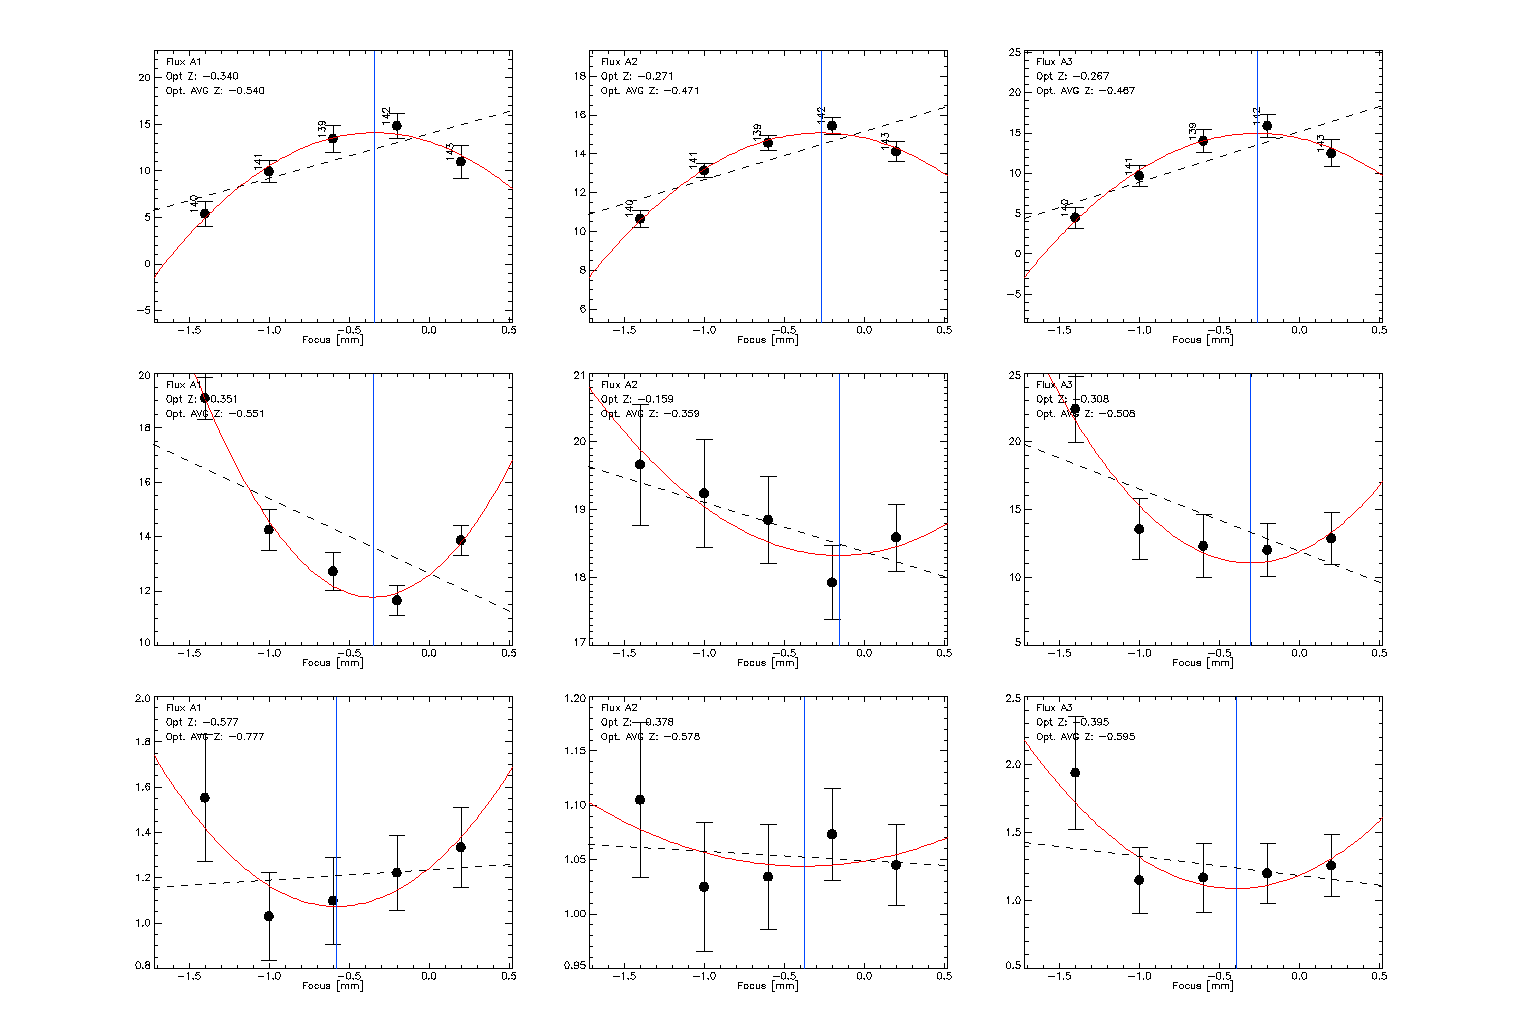
\includegraphics[clip, angle=0, trim={1.5cm, 1cm, 1.5cm, 1cm}, width=\textwidth]{Figures/plot_20170419s143.png}
\caption[Axial focus measure]{Example of axial focus measurement using a
  \emph{focus$\_$OTF} observation of Neptune during N2R10. The blue vertical line
  locates the optimal value of each fit. The optimal values derived from flux
  maximization and FWHM minimization agree to better than 0.1\,mm in these
  conditions of observation. While ellipticity may be regarded as a confirmation
  more than a decisive criterion (due to larger uncertainty on its measure), the
  associated minimum is also in good agreement with the values derived from flux
  and FWHM measurements.}
\label{fig:focus-example}
\end{center}
\end{figure}

The best axial focus in the central region of the arrays is estimated using the
so-called \emph{focus$\_$OTF} PAKO script, which produces a series of five $1'
\times 5'$ OTF scans at various values of the focus in $0.4~\rm{mm}$ steps
around an \emph{a priori} value $z_0$, namely $z \in \{-0.8, -0.4, 0, 0.4, 0.8\}
+ z_0$. Elliptical Gaussian fits on the reconstructed maps provide estimates of
the flux and FWHM along minor - and major - axes for each focus. Parabolic fits are
then used to determine the best focus. We consider three estimates: i) $\hat
z_{\rm{peak}}$ the focus that maximizes the estimated flux, which is the
amplitude of the 2D Gaussian, ii) $\hat z_{\rm{fwhm}}$ the focus that minimizes
the geometrical FWHM, defined as the quadratic mean of $\rm{FWHM}_{\rm{major}}$
and $\rm{FWHM}_{\rm{minor}}$, and iii) $\hat z_{\rm{ellipt}}$ the focus that
minimizes the beam ellipticity, defined as
$\rm{FWHM}_{\rm{major}}/\rm{FWHM}_{\rm{minor}}$. Fig.~\ref{fig:focus-example}
shows an example of such a sequence. When deciding on the focus to apply, we
give priority to the optimal flux, taking an average between values on A1 and
A3: there is little difference between the two, and the the 2\,mm channel is
less sensitive to focus than the 1\,mm.

As presented in more details in Sect.~\ref{sec:focus_surfaces}, the focus
surface is not strictly flat accross the FOV. The way sources are scanned in
this \emph{focus\_OTF} sequence is designed to save time but gives more weight
to the central KIDs. Hence, the optimal focus derived from the fits is
biased. To account for the curvature of the focus surfaces and optimize the
average focus accross the FOV, we add -0.2\,mm to the focus value as derived
in the previous paragraph.

\subsection{Lateral focus}
\label{sec:focus_X_Y}

Like in the $z$ (optical axis) direction, it is possible to control the position
of M2 along the $x$ and $y$ directions. We have tried to determine if there was
an optimal position in the $(x,y)$ plane that would improve further measures
with \nika. We have applied the same procedure as the one described in
Sect~\ref{se:axial_focus}, this time varying the position of M2 along $x$ or $y$
rather than along $z$. Examples of such observations are presented on
Figs.~\ref{fig:X_focus} and \ref{fig:Y_focus}. While the forced parabola fit
guides the eye towards optimization, one should note the size of the error bars
and the relatively low variations compared to M2 displacements along the $z$
axis. This is expected from optical simulations and experience on
EMIR. Figs.~\ref{fig:X_focus} and \ref{fig:Y_focus} also show as complement,
images of the residuals of the intensity maps at each M2 position after the
subtraction of an elliptical gaussian fitted only on a disk of 6 and 15\,arcsec
(1 and 2\,mm resp.) around the maximum location and outside a ring of 100\,arcsec
away from the maximum (to fix the background while not being affected by the
side lobes). These maps of residuals are meant to help decide on a minimization
criterion and $x$ or $y$-focus value.

While we have performed ``many'' such observations and explored the entire
parameter space of the $(x,y,z)$~triplet position in a reasonable range of
several millimeters around a fixed position, it has not been possible to
demonstrated that any $(x,y)$ position would improve significantly the
focalization of the whole system compared to the nominal $(0,0)$ reference
position. This confirms experience of the IRAM staff who only act on this
$(x,y)$ position about once a year after specific, dedicated and delicate
measures. We have therefore concluded that we should not change these parameters
for \nika\ and only rely on $z$-focus optimization for observations.

\begin{figure*}[h!]
\centering
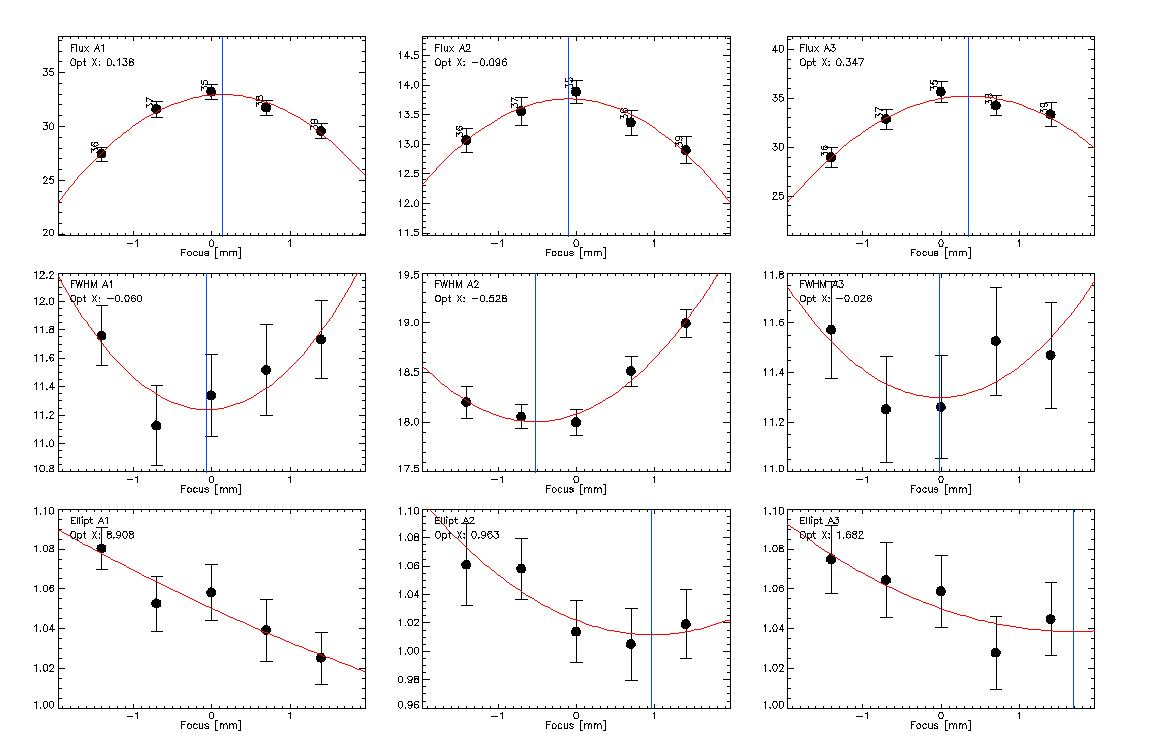
\includegraphics[height=8cm]{Figures/plot_20170223s39.png}
\hspace{0.5cm}
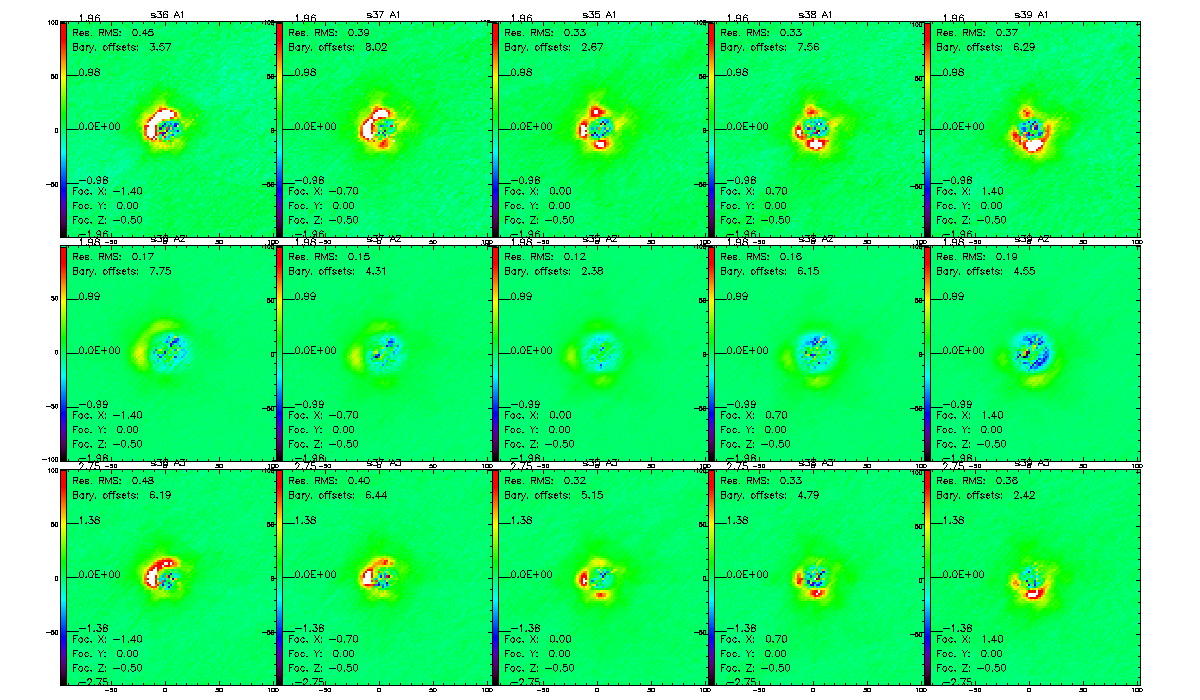
\includegraphics[height=8cm]{Figures/residuals_focus_otf_20170223s39.png}
\caption[Lateral X focus measures]{\textbf{Left:} X-focus measurement using a
    parabolic fit of the flux, beam fwhm and ellipticity on a sequence
    of five OTF scans on Uranus (20170223s39-43) \textbf{Right:} Beam residuals
    after subtracting a model of the main beam for each OTF-scan of the X-focus
    session. (N2R9)}
\label{fig:X_focus}
\end{figure*}

\begin{figure*}[h!]
\centering
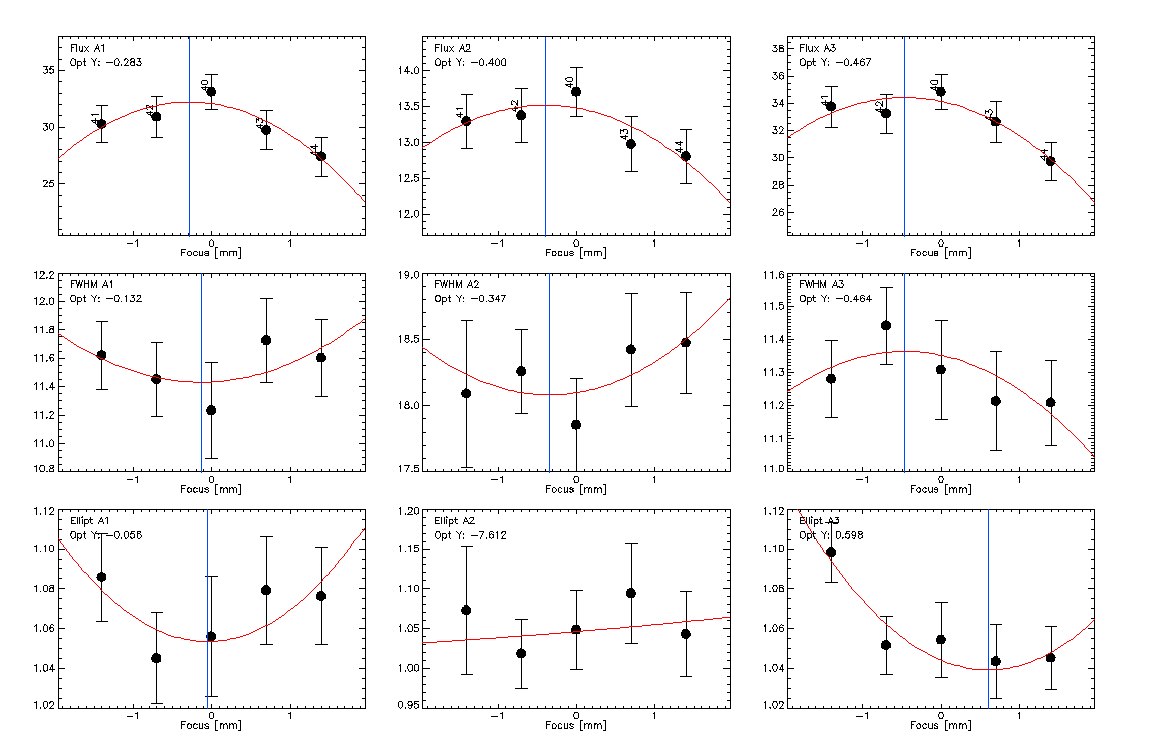
\includegraphics[height=8cm]{Figures/plot_20170223s44.png}
\hspace{0.5cm}
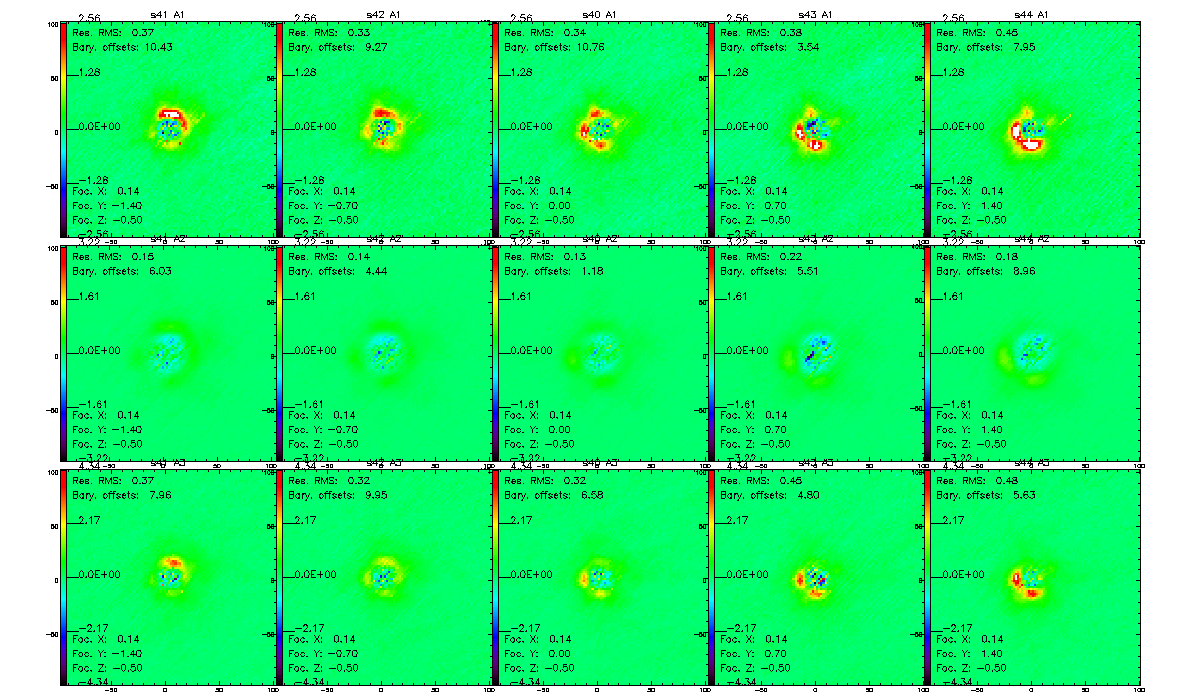
\includegraphics[height=8cm]{Figures/residuals_focus_otf_20170223s44.png}
\caption[Lateral Y focus measures]{\textbf{Left:} Y-focus measurement using a
    parabolic fit of the flux, beam fwhm and ellipticity on a sequence
    of OTF scans on Uranus (20170223s44-48). \textbf{Right:} Beam residuals
    after subtracting a model of the main beam for each OTF-scan of the Y-focus
    session. (N2R9)}
\label{fig:Y_focus}
\end{figure*}


\subsection{Pointing}
\label{se:pointing}
% + RTA pointing estimate method
% + pointing model
% + pointing error (scan-to-scan scattering)

Once the instrument is correctly focused, we can estimate pointing corrections
before scientific observations. The procedure that is used is very similar to
that used for EMIR and is described in the next subsection. It was used
repeatedly during pointing sessions to derive the pointing model of.

\paragraph{Pointing monitoring}

\begin{figure}[ht!]
\begin{center}
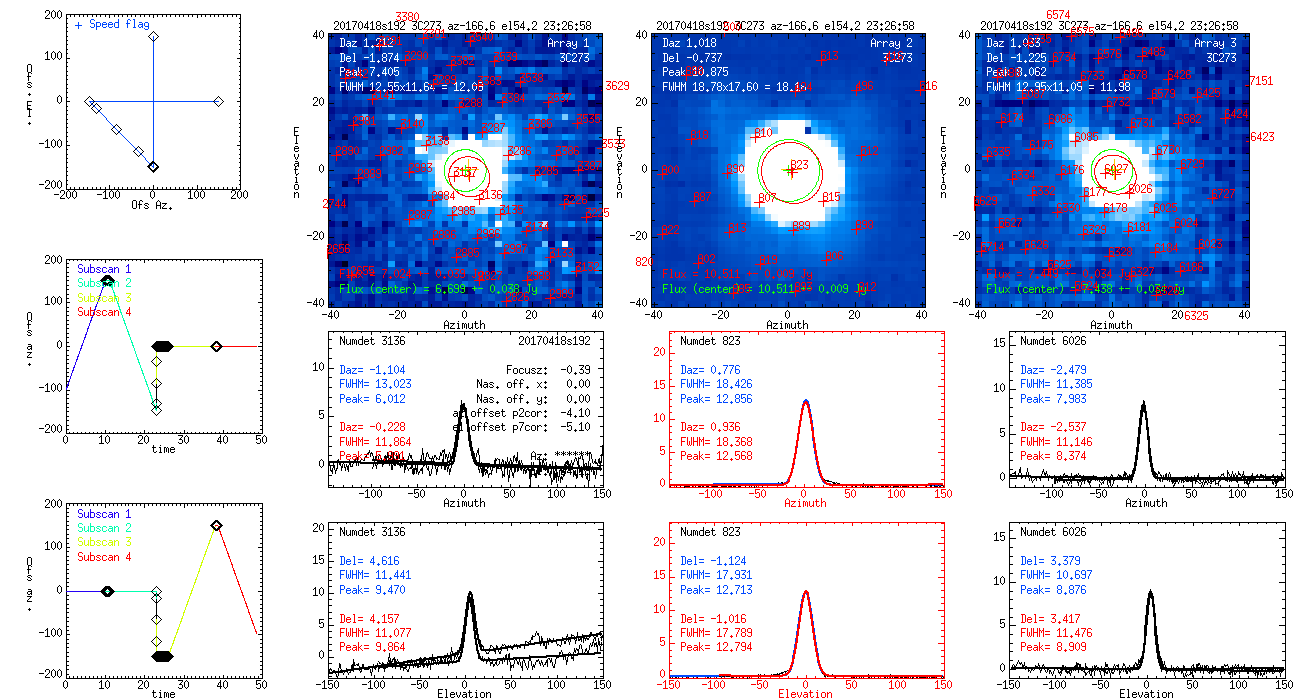
\includegraphics[clip, angle=0, scale = 0.30]{Figures/plot_20170418s192.png}
\caption[Summary plots of the reduction of pointing scan.]{There is one combined
  map per array to check the overall quality of the scan, and a set of azimuth
  and elevation profiles for one reference detector per array. The 2\,mm reference
  detector, highlighed in red, is the pointing reference detector of
  \nika. The location of the peak in azimuth and elevation, as observed by the
  reference detector gives the pointing offsets of the current scan.}
\label{fig:ptg}
\end{center}
\end{figure}

\begin{figure}[ht!]
\begin{center}
\includegraphics[clip, angle=0, trim={0, 0, 3cm, 0}, width=0.65\textwidth]{Figures/pointing_stats_N2R9.eps}
\caption[Pointing session results]{Pointing offsets during Run9 observations,
  before (blue to green) and after (yellow to red) the
  derivation of Nasmyth offsets with a pointing session on Feb.~26th, 2017.}
\label{fig:pointing_stats_n2r9}
\end{center}
\end{figure}

Based on general operating experience at the 30\,m telescope, we use the so-called
{\em pointing} or {\em cross} scans to monitor the pointing during observations. The
telescope executes a back and forth scan in azimuth and a back and forth scan in
elevation, centered on the observed source. Looking at the timeline profiles of
the reference detector, we fit gaussian profiles and derive the current pointing
offsets of the system in azimuth and elevation. These offsets can then be passed
to PAKO to recenter the next scan (Fig.~\ref{fig:ptg}).

\paragraph{Pointing session}
\label{se:pointing_session}

Such scans and their analyses are also used to improve the pointing model of
\nika. A pointing session consists in observing about 30 sources on a wide range
of elevations while monitoring the pointing offsets that are measured for each
observation. These offsets are then passed to the IRAM staff who finds the
pointing model parameters that minimize and symetrize the scattering of these
offsets. Bases on these results Nasmyth offsets are then
modified. Fig.~\ref{fig:pointing_stats_n2r9} shows the pointing corrections that
had to be applied during Run9, before and after the modification of the Nasmyth
offsets. The dispersion of the offsets is the figure of merit of the pointing
corrections. Their distribution after the corrections (in yellow to
red) is clearly more symmetric and narrower than before. During N2R9 run, the
pointing accuracy was 1.62\,arcsec rms in azimuth and 1.37\,arcsec rms in
elevation.

\subsection{Skydip}
\label{se:skydip}

A {\tt skydip} scan consists in a step-by-step span of a large range
of elevations.  This is used in order to calibrate the KIDs response
to the atmosphere for opacity derivation, as discussed in
Sect.~\ref{se:opacities}.  Namely, a skydip comprizes eleven steps in
the elevation range from 19 to 65 degrees, regularly spaced in
airmass. For each step, we acquire about twenty seconds of time traces
to ensure a precise monitoring of each KIDs. KIDs are tuned at the beginning of
each subscan (hence once per airmass). The variation of their resonnance
frequency reads

\begin{equation}
\ftone^k  = C_0^k - C_1^k T_{atm}[1-e^{-\tau/\sin\delta}]
\label{eq:skydip_1}
\end{equation}

An illustration is presented on Fig.~\ref{fig:ftone_vs_elev}. More details on
the analysis of these {\tt skydip} scans are given in Sect.~\ref{se:opacities}.

\begin{figure}[ht!]
\begin{center}
  \includegraphics[clip, angle=0, scale=0.75]{Figures/skydip_report.eps}
\caption[skydip]{Variation of the resonnance frequency of kid as a function of
  the elevation during a {\tt skydip} scan.}
\label{fig:ftone_vs_elev}
\end{center}
\end{figure}

\subsection{\bms}
\label{se:beammaps}

A \bm\ is a map of a bright and compact source, most of the time a planet, with
an elevation step small enough to meet Nyquist sampling of the 1\,mm beam,
namely 4.8~arcsec. We observe this planet with a raster scan in (az,el)
coordinates of $13\times7.8$~arcmin$^2$, either with fixed elevation subscans or
fixed azimuth subscans. The former has the advantage of low air mass variation
across a subscan, the latter offers an orthogonal scan direction to the former:
the combination of both gives a more accurate determination of the far side
lobes. The scan size ensures that the entire FOV is observed with good margins
for beam mapping even on the edges and good margin for baseline derivation and
subtraction in the scanning direction. During subscans, the telescope travels at
65\,arcsec/s. This values results of a compromise between the need to scan as
fast as possible to minimize atmospheric contamination while keeping subscans no
shorter than 10\,s (telescope constraint). The need to have Nyquist sampling of
the beams along the scan direction translates into a maximum speed 110\,arcsec/s
for our nominal acquisition rate of 23.8\,Hz and is thus largely met. Subscans
last 12\,s, the entire scan lasts about 25\,mn, which is short enough to prevent
to much variation of KID tuning under stable weather conditions on this
timescale.

More details on these observations are given in Sect.~\ref{se:fp_reconstruction}
where we describe how to actually exploit them to derive individual KID
properties.
